\section{Desarrollo protocolo de control in-band}
\label{sec:bofussDEV}


En esta sección se va a explicar la implementación realizada del protocolo Iotorii en el \textit{software switch} de \gls{bofus}. Dado que el trabajo de implementación ha sido bastante extenso, dado que había que discernir que parte de la implementación del control in-band podía ser aprovechada, se ha decidido generar un documento anexo \cite{davidBOFUSS} aparte de la memoria, donde se explique a bajo nivel las modificaciones realizadas. Todo el código se puede encontrar indicado en la Sección \ref{sec:estadoArte_github}. \\
\\
En la Figura \ref{fig:WIN-BOFUSS}, se puede apreciar la secuencia lógica que se ha llevado a cabo para la implementación del protocolo Iotorii en el software switch. En adelante se podrá encontrar el termino \texttt{win-BOFUSS}, el cual hará referencia a la implementación del protocolo Iotorii en la implementación de in-band del \gls{bofus}, conocida como \texttt{in-BOFUSS}, por lo que para añadirle la condición de \textit{wireless} se ha apodado como \texttt{win-BOFUSS}, del inglés \textit{\textbf{w}ireless \textbf{in}-band \textbf{B}asic \textbf{O}pen\textbf{F}low \textbf{U}serspace \textbf{S}oftware \textbf{S}witch}. En primer lugar, se han detectado todas las modificaciones realizadas anteriormente en la implementación del control in-band llevada a cabo por mi compañero Boby, y posteriormente se han clasificado en tres bloques funcionales: (1) Modificaciones del puerto local del ofprotocol, (2) Implementación de la  lógica de control del modo in-band, (3) Implementación del protocolo Amaru.\\
\\
Una vez se han identificado y se han clasificado todas las modificaciones realizadas sobre el \gls{bofus}, se va a pasar a la siguiente etapa, en la cual se va a ir módulo por módulo analizando y decidiendo si las modificacioens de cada módulo pueden ser aprovechadas en la implementación del \texttt{win-BOFUSS}. La primera modificación hacía referencia a un error en el tamaño del identificador del puerto local en el bloque de ofprotocol, tienendo que ser aplicado a 16 bits. Mi compañero, identificó que la lógica encargada de implementar el funcionamiento in-band del software-switch no se ejecutaba de manera adecuada. Se descubrió que este problema se debía a una discrepancia en el tamaño del identificador del puerto local, lo cual impedía que los datos correspondientes a dicho puerto fueran almacenados correctamente en la estructura utilizada por el módulo ofprotocol para almacenar los datos de los puertos del switch \gls{bofus}. Dichas modificaciones nos habría tocado hacerlas a nosotros, por lo que se han reaprovechado.\\
\\
Una vez reaprovechado dicho módulo de modificaciones, se ha seguido por el siguiente módulo el cual hace referencia a la implementación del control in-band del \textit{software switch}. En la implementación del \texttt{in-BOFUSS}, se detectó que el switch era incapaz de instalar reglas en las \textit{flow tables} de forma automatica en aras de mandar el tráfico de control OpenFLow por los puertos indicados. Esto se debía a que los mensajes encargados de instalar las reglas conocidos como \texttt{FLOW\_MOD}, generados de forma local, estaban siendo marcados como erróneos dado que estaban siendo mal generados, y por ello, el binario ofdatapath no podía instalar dichas reglas.

Más concretamente, la estructura de matches no se genera correctamente, por lo que el módulo ofdatapath es incapaz de extraer los matches e implementar adecuadamente las reglas a su tabla de flujos. El objetivo de estas modificaciones es lograr que el módulo ofprotocol sea capaz de crear mensajes FLOW\_MOD que permitan añadir las reglas necesarias para el funcionamiento en modo in-band, modificarlas o eliminarlas. Las principales modificaciones implementadas son:

\begin{itemize}
    \item Función make\_flow\_mod() del archivo ofp.c: Se crea correctamente la estructura de matches del paquete FLOW\_MOD y se rellenan los campos necesarios de los paquetes FLOW\_MOD. Para generar correctamente la estructura de match se ha implementado la función create\_ofl\_match\_UAH().

    \item Función make\_add\_flow() del archivo ofp.c: Se ha implementado la creación de un paquete FLOW\_MOD de tipo DROP, que instala una regla para descartar el flujo especificado en la estructura de match cuando el tamaño de las acciones sea 0, o un FLOW\_MOD normal en caso contrario.

    \item Función make\_add\_simple\_flow() del archivo ofp.c: Se ha modificado para que se cree un paquete FLOW\_MOD que instale una regla que encamine el tráfico, caracterizado por los campos de match, por un puerto concreto. Cuando el puerto de salida es 0, se crea un FLOW\_MOD del tipo DROP, es decir, una regla para descartar los paquetes del tráfico caracterizado por los campos de match.
\end{itemize}

% fig
\begin{figure}[ht]
    \centering
    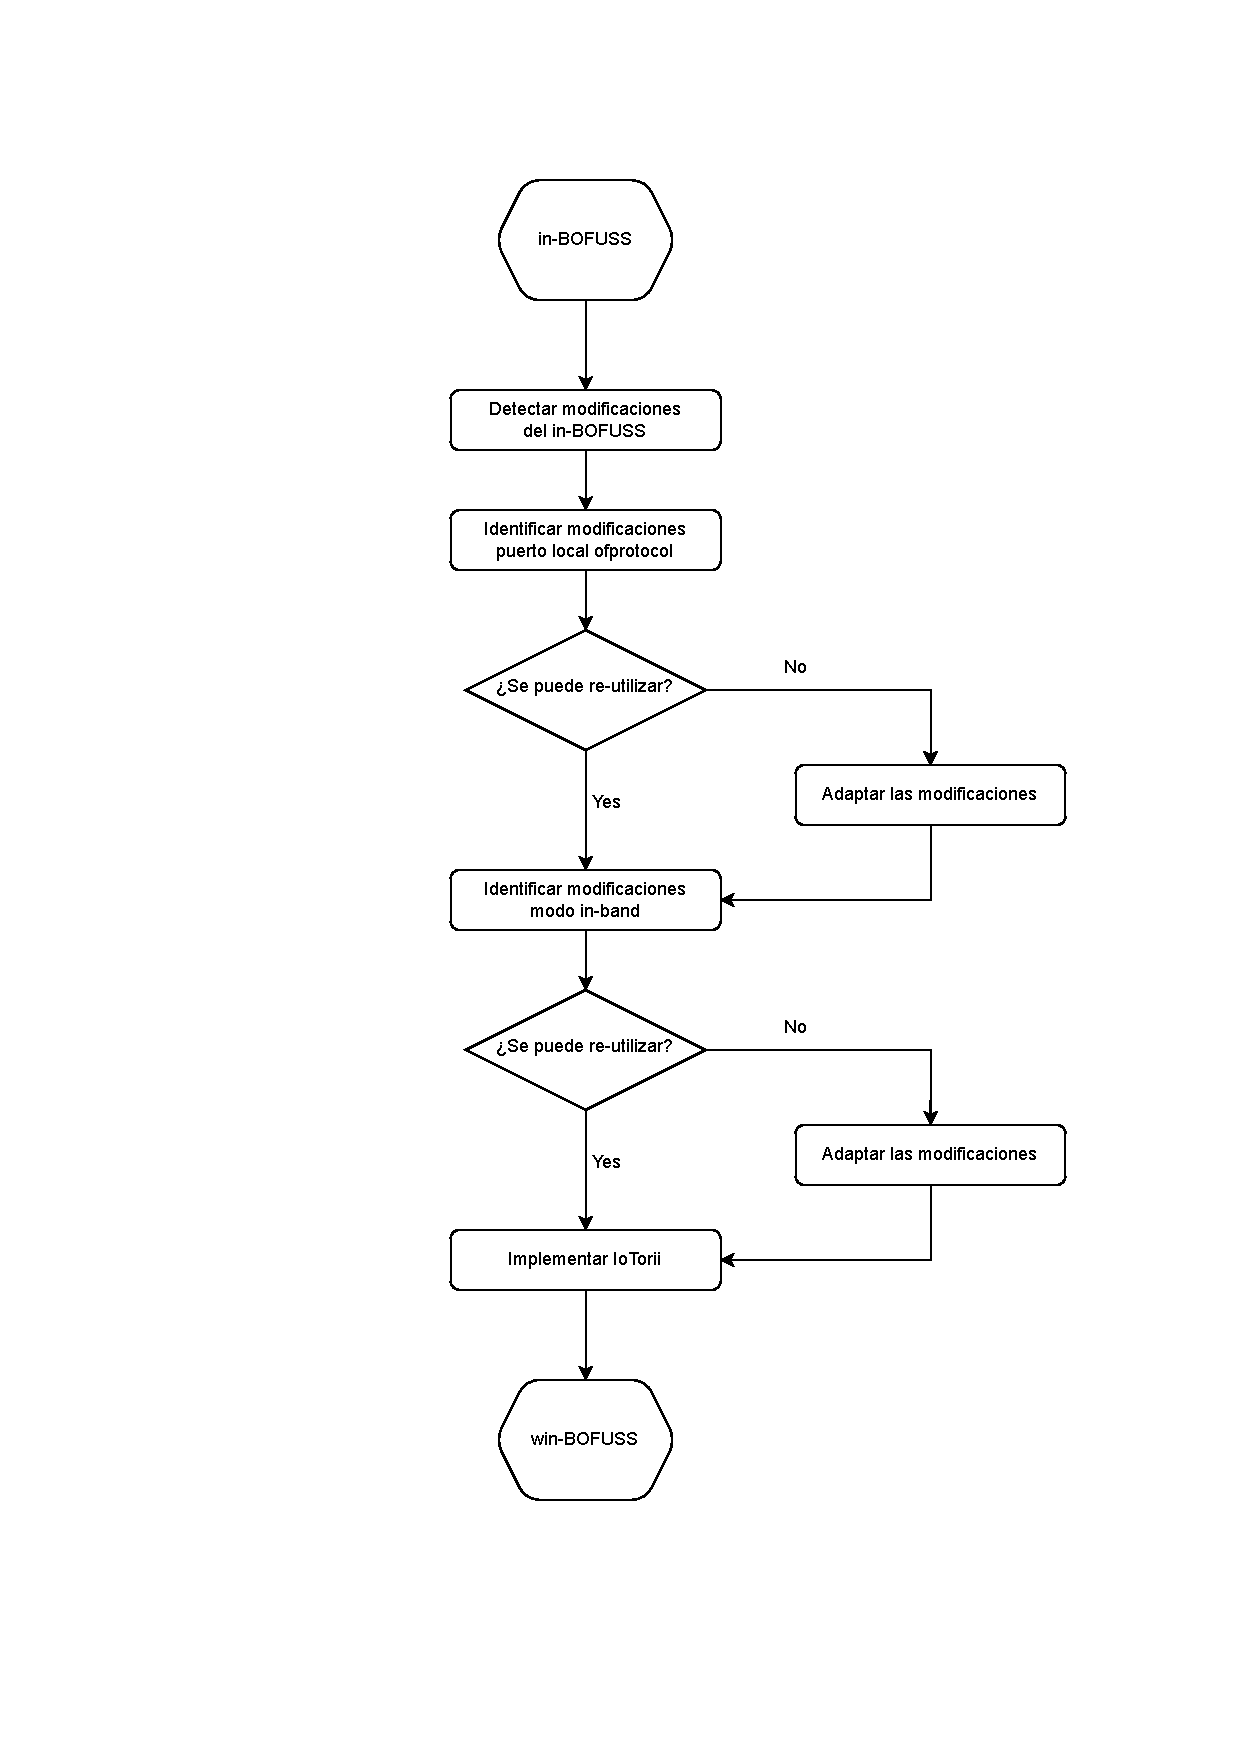
\includegraphics[width=\textwidth]{archivos/img/dev/WIN-BOFUSS.drawio.pdf}
    \caption{Diagrama de flujo para la implementación del protocolo Iotorii en el software switch \glsentryshort{bofus}}
    \label{fig:WIN-BOFUSS}
\end{figure}


